% Created 2016-09-12 Mon 20:22
\documentclass[11pt]{article}
\usepackage[utf8]{inputenc}
\usepackage[T1]{fontenc}
\usepackage{fixltx2e}
\usepackage{graphicx}
\usepackage{grffile}
\usepackage{longtable}
\usepackage{wrapfig}
\usepackage{rotating}
\usepackage[normalem]{ulem}
\usepackage{amsmath}
\usepackage{textcomp}
\usepackage{amssymb}
\usepackage{capt-of}
\usepackage{hyperref}
\author{William Henney}
\date{\today}
\title{Plane parallel steady state flow from blackboard notes}
\hypersetup{
 pdfauthor={William Henney},
 pdftitle={Plane parallel steady state flow from blackboard notes},
 pdfkeywords={},
 pdfsubject={},
 pdfcreator={Emacs 24.5.2 (Org mode 8.3.5)}, 
 pdflang={English}}
\begin{document}

\maketitle
\tableofcontents

\begin{itemize}
\item Initial equations
\begin{itemize}
\item \(\rho v = \Phi_{0} \equiv \rho_{1} v_{1}\)
\item \(\rho \, (a^{2} + v^2) = \Pi_{0} \equiv \rho_{1} a_{1}^{2} \, (1 + M_{1}^{2})\)
\item \(\frac52 \rho v a^{2} \, (1 + \frac15 M^{2}) = \mathcal{E}_{0} - \int L\, dx\)
\begin{itemize}
\item where \(\mathcal{E}_{0} \equiv \frac52 \rho_{1} v_{1} a_{1}^{2 }\, (1 + \frac15 M_{1}^{2})\)
\end{itemize}
\end{itemize}
\item Can be boiled down to
\begin{enumerate}
\item \((1 + M^{2}) \, a^{2}/v = \Pi_{0}/\Phi_{0} = (1 + M_{1}^{2}) \, a_{1}^{2}/v_{1} = (1 + M_{0}^{-2}) \, v_{0}\)
\begin{itemize}
\item This is how velocity varies with soundspeed
\item For subsonic limit (\(M^{2} \ll 1\)) it is effectively \(v \propto a^{2}\).  If the particle mass is not changing (constant ionization) then this is \(v \propto T\)
\end{itemize}
\item \(a^{2} \, (1 + \frac15 M^{2}) = a_{1}^{2} \left( 1 + \frac15 M_{1}^{2} - \frac32 \int \mathcal{L} \, ds \right)\)
\begin{itemize}
\item This is how the sound speed (or Temperature) varies with distance
\item Where \(\mathcal{L} = L / L_{1}\) is dimensionless cooling function
\item \(s = x / h\) is dimensionless distance in terms of the cooling length: \(h = \frac35 \rho_{1} a_{1}^{2} v_{1} / L_{1}\)
\item And the immediate post-shock cooling function is \(L_{1} = n_{1}^{2} \Lambda(T_{1})\)
\end{itemize}
\end{enumerate}
\end{itemize}
\section{Try to solve the subsonic-limit case and with power law cooling func}
\label{sec:orgheadline1}
\begin{itemize}
\item Assume \(\Lambda = \Lambda_1 (T/T_1)^a\), where \(a \approx -1\) for 10\(^{\text{5}}\) to 10\(^{\text{6}}\) K
\item So first equation gives \(v/v_1 = T/T_1\) and \(n/n_1 = T_1/T\)
\begin{itemize}
\item => \(\mathcal{L} = (n/n_1)^2 (T/T_1)^a = (T/T_1)^{a-2 }\)
\end{itemize}
\item And second equation gives
\begin{itemize}
\item \(\tau = 1 - 1.5 \int \tau{}^{a-2 }\, ds\)
\item where \(\tau \equiv T/T_1\) is the dimensionless temperature
\item Differentiating: \(d\tau/ds = -1.5 \tau{}^{a-2 }\)
\begin{itemize}
\item => \(\int_1^\tau \tau^{2-a}\, d\tau = -1.5 \int_0^s ds\)
\item => \((\tau^{3-a} - 1) / (3-a) = -1.5 s\)
\item => \(\tau = (1 - 1.5 (3-a) s)^{1/(3-a)}\)
\end{itemize}
\item For example, with \(a = -1\)
\begin{itemize}
\item \(\tau = (1 - 6 s)^{1/4 }\)
\end{itemize}
\item For example, with \(a = +2\)
\begin{itemize}
\item \(\tau = 1 - 1.5 s\)
\end{itemize}
\end{itemize}
\end{itemize}

\begin{verbatim}
####+BEGIN_SRC python :results file :return pltfile
import numpy as np
from matplotlib import pyplot as plt
pltfile = 'cooling-shell.pdf'
fig, ax = plt.subplots(1, 1)
s = np.linspace(0, 0.167, 500)
a = -1
tau = (1.0 - 1.5*(3 - a)*s)**(1./(3 - a))
print(tau)
rho = np.nanmin(tau)/tau
print(rho)
ax.plot(s, tau)
ax.plot(s, rho)
ax.set_ylim(0, 1)
fig.savefig(pltfile)
\end{verbatim}

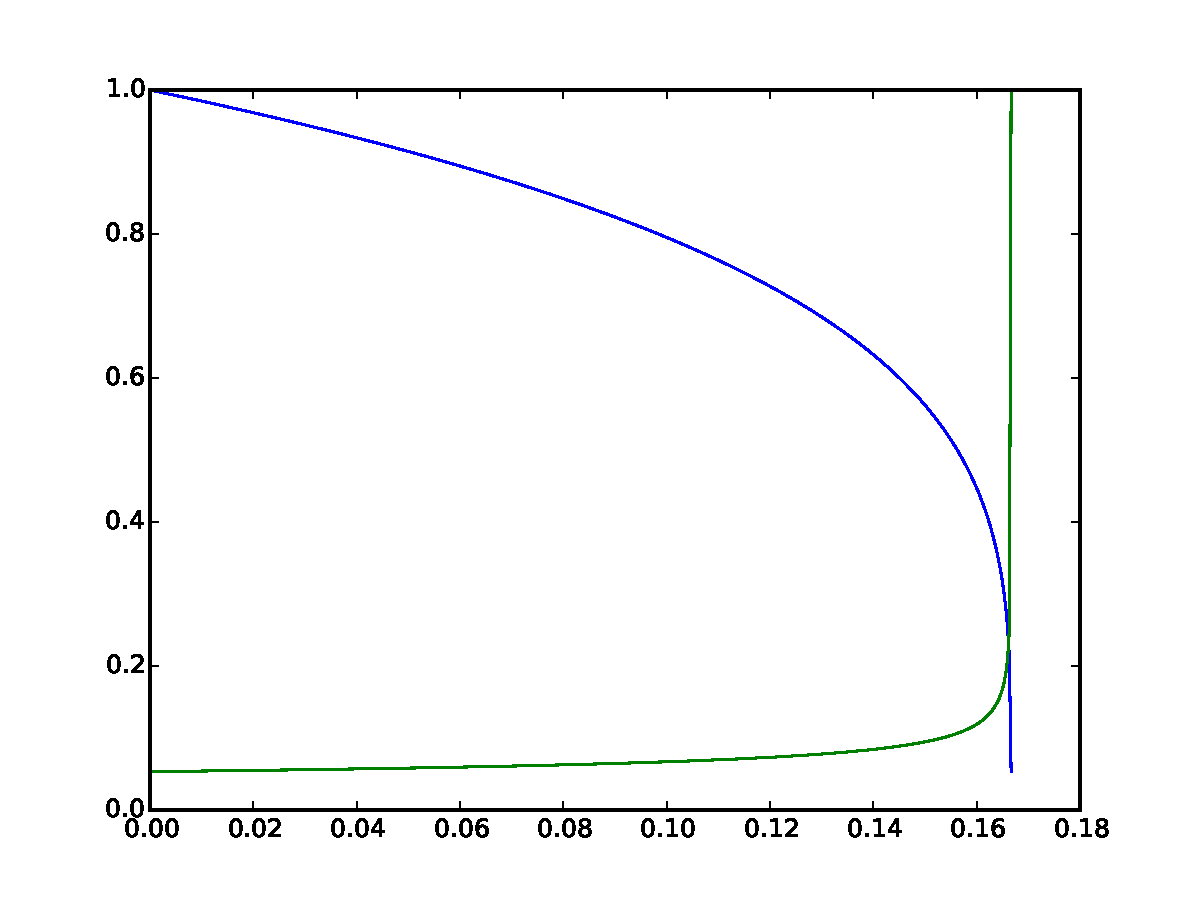
\includegraphics[width=.9\linewidth]{cooling-shell.pdf}
\section{Use real cooling function instead}
\label{sec:orgheadline2}
:ID:       05FA6299-E408-4935-8237-194ECCA91844
\begin{itemize}
\item This is an attempt to reconstruct this from memory since I had an emacs disaster last night and lost all my work for the last two days
\item First equation is the same
\item Second equation is \(T / T_{1} = 1 - 1.5 \int (\Lambda / \Lambda_{1})(T_{1}^{2}/T^{2})\, ds\)
\begin{itemize}
\item Differentiating: \((1/T_{1}) dT/ds = -1.5 (\Lambda / \Lambda_{1})(T_{1}^{2}/T^{2})\)
\item => \(s = \frac23 (\Lambda_{1}/T_{1}^{3}) \, \int_{T}^{T_{1}} (T^{2} / \Lambda) \, dT\)
\end{itemize}
\item Note that the following needs to be run in python 3
\end{itemize}
\begin{verbatim}
import os
import numpy as np
from scipy import interpolate, optimize, integrate
from astropy.table import Table
from matplotlib import pyplot as plt
import seaborn as sns

def get_cooltable(logphi=10.0, logn=0.0, star='wr136', cwd='.'):
    cooldir = os.path.join('JaneCloudy', star.upper() + 'COOL/')
    templ = 'coolfunc-photo-{}-phi{:.2f}-ngc6888-n{:.2f}.dat'
    coolfile = templ.format(star, logphi, logn)
    return Table.read(os.path.join(cwd, cooldir, coolfile),
                      format='ascii.commented_header', delimiter='\t')

# Set up cooling function
tab = get_cooltable()
T_tab = tab['Temperature']
Lambda_tab = (tab['L (erg/cm3/s)'] - tab['H (erg/cm3/s)'])/(tab['Np']*tab['Ne'])
fLambda = interpolate.interp1d(T_tab, Lambda_tab)

# Calculate integral on finer grid
integrand_tab = T_tab**2 / Lambda_tab
fIntegrand = interpolate.interp1d(T_tab, integrand_tab)

# Equilibrium T where heating = cooling
Teq = optimize.fsolve(fLambda, 1e4)
# Go up to 1e6 K
logThi = 6.0
# And down to just above equilibrium T
logTlo = np.log10(1.001*Teq)
ngrid = 50
T_grid = np.logspace(logTlo, logThi, ngrid)

Lambda_grid = fLambda(T_grid)
# integrand_grid = fIntegrand(T_grid)

# Don't interpolate the integrand - rather recalculate it from the
# interpolated T and Lambda
integrand_grid = T_grid**2 / Lambda_grid
integral_grid = integrate.cumtrapz(integrand_grid, T_grid, initial=0.0)
fIntegral = interpolate.interp1d(T_grid, integral_grid)

# Set up graph for temperature and density
pltfile = 'cooling-shell-new-n100.pdf'
fig, (axtop, axbot) = plt.subplots(2, 1, sharex=True)

# Loop over all the shock velocities
for row in models:
    M0, u0, v1, n0, n1, N2, T1, dcool, tcool = [float(x) for x in row]
    label = 'Vs = {:.0f} km/s'.format(u0)
    mask = T_grid < T1
    T = T_grid[mask][::-1]
    s = (2./3.)*(fLambda(T1)/T1**3)*(fIntegral(T1) - integral_grid[mask][::-1])
    x = np.hstack([[-0.05, 0.0, 0.0], dcool*s]) 
    axtop.semilogy(x, np.hstack([[Teq, Teq, T1], T]))
    den = n1*T1/T
    axbot.semilogy(x, np.hstack([[n0, n0, n1], den]), label=label)

axtop.set_ylim(9000, 1.1e6)
axbot.set_ylim(0.3, 200.0)
axbot.set_xlabel('Distance, pc')
axbot.set_ylabel('Density, pcc')
axtop.set_ylabel('Temperature, K')
axbot.legend(ncol=3, fontsize='x-small', loc='upper center')
fig.savefig(pltfile)

#return list(zip(T_grid, Lambda_grid, integrand_grid, integral_grid))
\end{verbatim}

\section{[O III] and Ha emissivities}
\label{sec:orgheadline5}

\subsection{Equilibrium emissivity in the cooling zoone}
\label{sec:orgheadline3}

\subsection{Non equilibrium emissivity in the shock}
\label{sec:orgheadline4}




\section{Relation of isothermal sound speed and temperature:}
\label{sec:orgheadline6}
\begin{itemize}
\item \(\rho\) a\(^{\text{2}}\) = n\(_{\text{tot}}\) k T
\item \(\rho\) = m\(_{\text{p}}\) n\(_{\text{H}}\) (1 + 4 y\(_{\text{He}}\))
\item n\(_{\text{tot}}\) = n\(_{\text{H}}\) (1 + x\(_{\text{H}}\) + y\(_{\text{He}}\) (1 + x\(_{\text{He}}\) + 2 x\(_{\text{HeII}}\)))
\item => a\(^{\text{2}}\) = (k / \(\mu\) m\(_{\text{p}}\)) T
\begin{itemize}
\item where \(\mu\) = (1 + 4 y\(_{\text{He}}\)) / (1 + x\(_{\text{H}}\) + y\(_{\text{He}}\) (1 + x\(_{\text{He}}\) + 2 x\(_{\text{HeII}}\)))
\end{itemize}
\item Table of \(\mu\) values
\begin{center}
\begin{tabular}{rrrr}
y\(_{\text{He}}\) & x\(_{\text{H}}\) & x\(_{\text{He}}\) & \(\mu\)\\
\hline
0.1 & 0.0 & 0.0 & 1.27\\
0.1 & 1.0 & 0.0 & 0.67\\
0.1 & 1.0 & 1.0 & 0.64\\
\hline
0.162 & 0.0 & 0.0 & 1.42\\
0.162 & 1.0 & 0.0 & 0.76\\
0.162 & 1.0 & 1.0 & 0.71\\
\end{tabular}
\end{center}
\end{itemize}
\end{document}
